\documentclass[sigchi, review]{acmart}

\usepackage{booktabs} % For formal tables

% Copyright
%\setcopyright{none}
%\setcopyright{acmcopyright}
%\setcopyright{acmlicensed}
%\setcopyright{rightsretained}
%\setcopyright{usgov}
%\setcopyright{usgovmixed}
%\setcopyright{cagov}
\setcopyright{licensedcagov}
%\setcopyright{cagovmixed}
%\setcopyright{licensedothergov}

% DOI
\acmDOI{10.475/123_4}

% ISBN
\acmISBN{123-4567-24-567/08/06}

%Conference
\acmConference[Literature Review'18]{CHI 2018}{July 2018}{Pathum Thani TH}
\acmYear{2018}
\copyrightyear{2018}

\acmPrice{15.00}


\begin{document}
\title{Literature Review(LOL Streakiness,Coco's videos,G2G)}
\titlenote{Produces the permission block, and
  copyright information}
\subtitlenote{The full version of the author's guide is available as
  \texttt{acmart.pdf} document}



\author{Chatphimuk Supinyo}
\affiliation{%
  \institution{Thammasat University}
  \streetaddress{30 Shuangqing Rd}
  \city{Pathum Thani}
  \country{Thailand}
}



\begin{abstract}
This paper is Literature Review that will explain about 3 research paper 1.)Playing with Streakiness in Online Games: How Players
Perceive and React to Winning and Losing Streaks in League of Legends 2.)Coco’s Videos: An Empirical Investigation of Video-Player
Design Features and Children's Media Use 3.)G2G: The Design and Evaluation of a Shared Calendar and
Messaging System for Grandparents and Grandchildren  
\end{abstract}



\keywords{League of Legends,Strekiness,Coco's videos,G2G(Grandparents-to-Grandchildren),ACM proceedings, \LaTeX, text tagging.}

\begin{teaserfigure}
  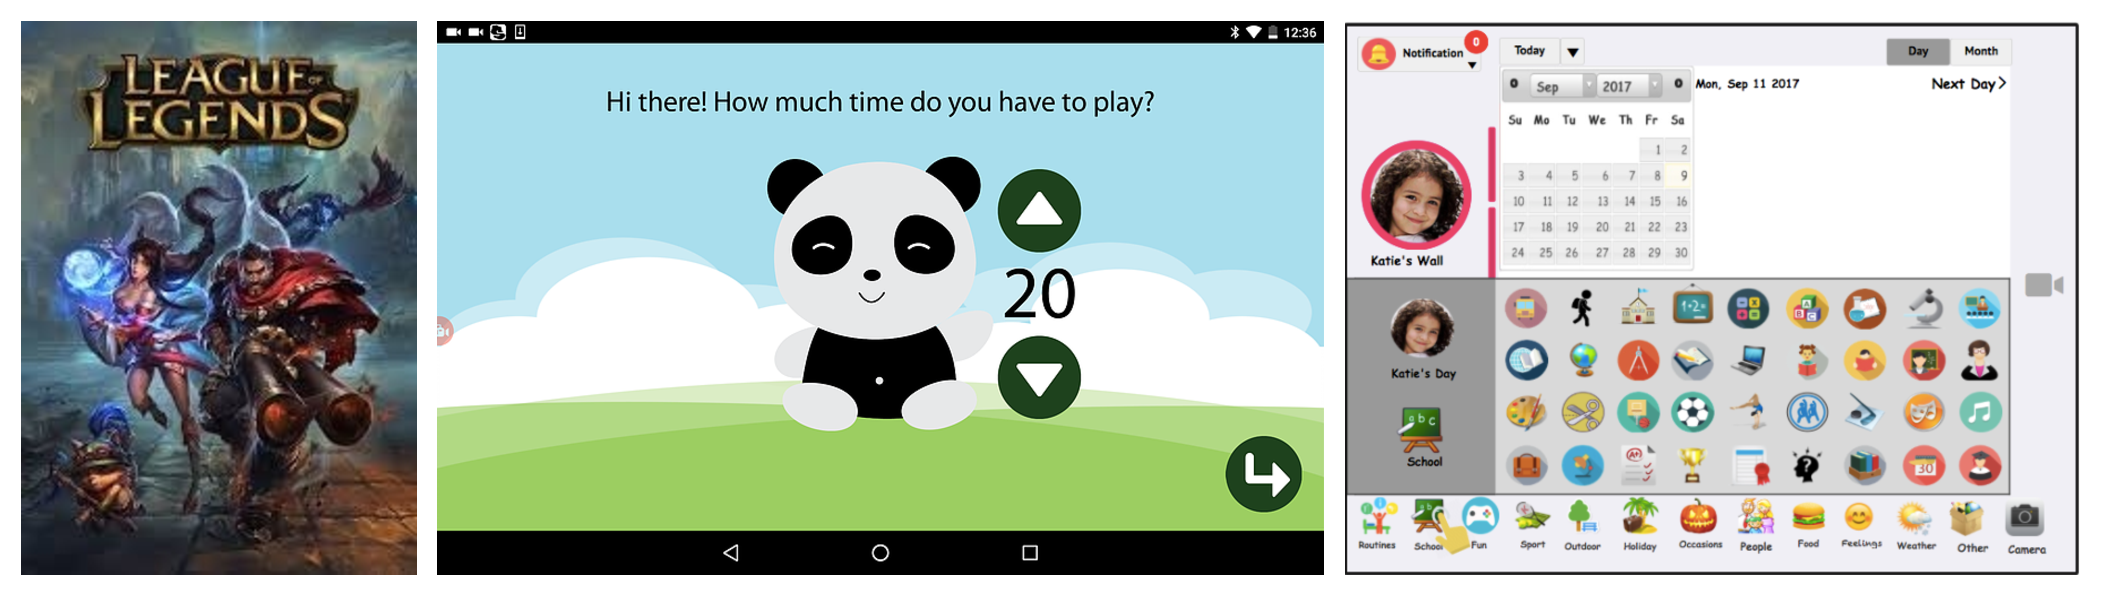
\includegraphics[width=\textwidth]{sampleteaser}\Description{A
    baseball field}
  \caption{This is a picture of LOL,Coco videos and G2G}
  \label{fig:teaser}
\end{teaserfigure}


\maketitle

\section{Literature Abstract}


\subsection{Playing with Streakiness in Online Games: How Players
Perceive and React to Winning and Losing Streaks in
League of Legends }

Streakiness refers to observed tendency towards
consecutive appearances of particular patterns. In video
games, streakiness is oftentimes inevitable, where a player
keeps winning or losing for a short period. However, the
phenomenon remains understudied in present online game
research. How do players perceive streakiness? How does it
impact player experience (PX)? How should streakiness be
taken into consideration for the design of PX? In this paper,
we address these questions through a qualitative study of
player discussions about streakiness in League of Legends.
We found that players developed various ways to describe a
streak. Both winning and losing streaks negatively impacted
PX. Players devised numerous strategies to manage
streakiness, among which disengagement was a primary
means. We analyze streakiness as a social construct through
which players coped with complex game systems. We
discuss design implications for managing streakiness in
online games.

\subsection{Coco’s Videos: An Empirical Investigation of Video-Player
Design Features and Children's Media Use }

In this study, we present Coco’s Videos, a video-viewing
platform for preschoolers designed to support them in learning to self-manage their media consumption. We report results from a three-week experimental deployment in 24
homes in which preschoolers used three different versions of
the platform: one that is neutral to the limits they set, one that
enforces the limits they set, and one that attempts to erode
the limits they set by automatically playing additional content after the planned content is finished (“post-play”). We
found that post-play significantly reduced children’s autonomy and likelihood of self-regulation, extended video-viewing time, and led to increases in parent intervention. We
found that the lock-out mechanism did not reduce videoviewing time or the likelihood of parent intervention. Together, our results suggest that avoiding platforms that work
to undermine the user’s intentions is more likely to help children self-regulate their media use than rigid parental controls.


\subsection{G2G: The Design and Evaluation of a Shared Calendar and
Messaging System for Grandparents and Grandchildren }

Distance separated grandparents and grandchildren often
face challenges in staying connected. To explore this topic,
we designed G2G, a shared calendar and video messaging
system to connect young children (ages 5-10) with their
grandparents over distance. Our design focused on
providing grandparents and grandchildren with an
awareness of each other’s lives to support conversations
and design elements to help reduce the need for parent
scaffolding. A field study with two grandparent-grandchild
pairs over two months showed that systems designed
around structured communication can help young children
develop a routine around staying in touch with their remote
grandparents. Autonomy in maintaining awareness can help
children to be engaged more easily. This suggests that
designs focusing on connecting young children to their
grandparents over distance should be flexible yet structured
and designing to reduce parental scaffolding can lead to
positive effects and strengthened relationships.

\section{Literature Introduction}

\subsection{Playing with Streakiness in Online Games: How Players
Perceive and React to Winning and Losing Streaks in
League of Legends }

Streakiness, which this paper defines as observed tendency
towards consecutive appearances of particular patterns
(such as wins or losses), is commonly observed and
discussed in the literature on sports  and gambling .
While decades of research on streakiness remains
inconclusive in the existence of such phenomenon and to 
what extent it can be attributed to randomness
, people themselves often make welldeveloped
interpretations of this phenomenon and adjust
their behaviors accordingly . Superstitious practices
might ensue after experiences with streaks: people fear that
certain actions will wash away their good luck after a
winning streak, but believe that certain actions will wash
away bad luck after a losing streak .


Similar to sports and gambling, competitive online games
involve win or loss and therefore contain winning or losing
streaks as a natural component of player experience (PX).
However, little game research in human-computer
interaction (HCI) has considered the PX with streakiness in
competitive online games. Since players’ interpretation and
explanation of achievement and failure significantly impact
PX , it is important to understand how players make
sense of streaks, and how streaks impact PX.


We studied streakiness in League of Legends (LoL) to
answer three research questions: 1, what is considered a
streak, 2, what causes streaks, and 3, how players react to
streaks? We used content analysis to examine player
discussions about streaks from two LoL-focused forums
(i.e., the LoL boards and the LoL subreddit). We found that
players used four factors (number of wins/losses, ranking
score, time, and win rate) to determine whether they were
experiencing streaks. Players developed various theories to
explain streakiness, ranging from personal skill and ingame
performance to the design of matchmaking system.


Losing streaks negatively impacted PX and reduced player
engagement. Players reported enjoying winning streak, but
would also develop anxiety with the belief that a losing
streak might ensue. Streakiness thus plays a critical role in
PX. We consider how player discourses constructed
streakiness through sensemaking, which refers to
“placement of items into frameworks, comprehending,
redressing surprise, constructing meaning, interacting in
pursuit of mutual understanding, and patterning”. Our
contributions include bridging game research with
streakiness studies in the sports and gambling literature,
systematically documenting PX with streakiness, providing
an in-depth analysis of the streakiness phenomenon in LoL,
and deriving design implications from the perspective of
sensemaking. 


\subsection{Coco’s Videos: An Empirical Investigation of Video-Player
Design Features and Children's Media Use }

Entertainment media plays a central role in the lives of young
children, with the average preschooler watching more than
three hours of television, film, and other video programming
each day . Children’s television and videos can provide productive learning opportunities for kids  and useful respites from caregiving for adults , in addition to
serving as an enjoyable part of daily life. However, child development research also suggests families set limits on the
amount of time preschoolers spend consuming passive video
content, as heavy viewing has been linked to increased risk
of obesity , reductions in imaginative play , and sleep
disruption . In addition, the low cognitive demand and
high-reward experience of viewing videos make it easy for
viewers to engage in extended consumption .


In this study, we examine the role of design as it relates to
children’s transitions to and from video viewing experiences.
As part of this, we investigated two different existing design
paradigms with the potential to influence children’s transition behaviors. First, a variety of commercial products
known as “parental controls” offer to support parents in setting and enforcing limits on children’s use of technology, including controls specifically targeting video viewing .
Second, in direct contrast to the limit-enforcing goals of parental controls, many popular platforms serving videos include post-play features and next-video suggestions that seek
to promote continued viewing and minimize natural stopping
points by automatically playing new content when the selected video ends. Prior work has shown that parents find
post-play and related features frustrating and believe these
impede their family’s ability to set boundaries .


The extent to which either limit-enforcing (parental controls)
or limit-eroding (post-play) designs influence families’ behaviors in practice is not robustly understood. Prior work
suggests that the authoritarian design and rigidity of parental
controls are unlikely to best serve families’ needs ,
while other work has shown that these interfaces are often
poorly understood and difficult to use . To the best of
our knowledge, no prior work has examined the effect postplay in the context of limit-setting, despite the fact that it is a
common feature of Internet video-on-demand platforms such
as Netflix and YouTube.


We undertook the current project in pursuit of two specific
goals. The first was to build on our past design work to
create a video-viewing platform to support preschoolers in
planning their media consumption with intention. The second was to conduct an experimental study to understand how
designs intended to either enforce or erode families’ limits
influence parents’ and children’s experiences with this system in a real-world context. To do this, we created “Coco’s
Videos,” which we deployed in the homes of 24 families with
preschoolers for three weeks. We conducted a within-subjects comparison of families’ responses to three different versions of the system. In these conditions, the platform alternatively: 1) remained agnostic to families’ limits, 2) actively
attempted to enforce families’ limits with a lock-out mechanism, or 3) actively attempted to undermine families’ limits
with a post-play mechanism.


We found, first, that children engaged with the core experience with intention and displayed autonomous decisionmaking as they planned their video viewing. In addition,
children took ownership of their transition experience as they
ended their viewing and moved on to other activities. Second, we found that post-play extended children’s viewing
time, led to increased intervention from parents, reduced evidence of children’s autonomy, and was perceived negatively
by parents relative to the other versions of the system. Third,
we found that the lock-out mechanism did not appear to reduce children’s autonomy, although it also did not reduce
viewing time or increase the need for parents to intervene.
As media corporations increasingly seek to engage and monetize the attention of their preschool audience , it is useful
for the design community to understand how specific design
choices influence children’s patterns of engagement and disengagement. While children’s media plays a positive role in
daily life for many, families’ usage patterns will always necessarily include both disconnecting and connecting. The contribution of this work is to support designers in understanding how their choices may influence children’s ability to autonomously self-regulate their use of media and parents’ selfefficacy in supporting their children’s media habits


\subsection{G2G: The Design and Evaluation of a Shared Calendar and
Messaging System for Grandparents and Grandchildren }

Technology has provided a variety of ways for distanceseparated family members to maintain connections over
distance. Yet many families still face challenges in building
strong emotional bonds between young children and their
grandparents over distance .
Video applications such as Skype and FaceTime have
improved remote communication with children
however, children’s limited attention span makes it
cumbersome to keep them engaged in remote conversation
at young ages. Thus, maintaining regular frequent phone
calls or video calls between young children and remote
grandparents which satisfy all can be a challenge . As a
result, most research in this area has focused on connecting
young children with their grandparents through sharing a
limited set of activities rather than direct conversation
. 

While beneficial, these systems mostly direct
communication to focus on superficial exchanges, rather
than more detailed information that might help
grandparents and grandchildren feel closer despite the
distance between them . Such information might include
personal stories and daily life experiences, which might
help grandparents feel confident during communication .
In this paper, we present the design of a communication
system for distance-separated grandparents and young
grandchildren called G2G (Grandparents to Grandchildren).
G2G is a shared calendar and video messaging system
designed to help grandparents and grandchildren (5-10
years old) maintain an awareness of each other’s daily lives
through a simple and playful calendar while communicating
asynchronously through video messages. We hoped that a
mutual awareness of each other’s lives, gained through the
system could act as a catalyst to promote communication
between grandparents and grandchildren.
Next, we conducted a field evaluation of G2G with an
emphasis on middle class, heterosexual families with two
parent-households. Our research questions focused on how
distance-separated grandparents and young grandchildren
would use it to communicate over distance; if and why such
a system would change their communication behavior; and,
what benefits and challenges families would find in such a
system. Our goal was to understand what design factors
were important for mutual awareness and communication
between grandparents and grandchildren. 

Our deployment
was conducted with two pairs of families—including a total
of eight adults and four children—for eight weeks.
Our evaluation revealed that both grandparents and
grandchildren valued G2G and were able to incorporate it
into their communication and establish new routines for
staying connected. The structured nature of communication,
as facilitated by the system, made this possible as did the
emphasis on providing mutual awareness of one’s life.
However, both grandchildren and grandparents wanted
features that might help them develop closer relationships
with individuals, such as targeted messaging. They also
desired communication mediums that were expressive and
lightweight. Together, these findings point to design
implications for the creation of technologies to support
grandparent-grandchild communication over distance, with
an emphasis on awareness and context

\section{Literature Review and Conclusion}

\subsection{Playing with Streakiness in Online Games: How Players
Perceive and React to Winning and Losing Streaks in
League of Legends }

This paper is talk about Strekiness in LOL( League of Legends )online game and how player react when they get streakiness(Winning streaks and Losing streaks)
What is difference about both streaks.They collect data from 2 place first is League of Legends official forum and second is Reddit Forum andthey use key word "Streak" to find data that they want to analyse it.

The conclusion in this  paper is in both streaks players will show they bad react in losing streak they feel sad,fear and angry when they lose.In winning streak they feel not good because when they win more they feeling 
losing strek will coming too and they will lose of their confidence to play game again.

\subsection{Coco’s Videos: An Empirical Investigation of Video-Player
Design Features and Children's Media Use }

In this paper is talk about Coco's Videos.It's a android application that make to help about Internet Addict when kids watch Videos on YouTube.This application will alert when kids is watch videos end Coco character will show and talk to them(kids) for they should do activity
before watch next video.The experiment in this paper they do with 28 families. The design of Coco's Videos have three diffence design: 

1.)neutral this design is very simple it's has a one features that is Home Button 

2.)post-play this design it's has a Home button like a neutral but in this desgin will have a video's trailer on the top left of the screen 
 
3.)controlled. this design it's not has a feature like a neutral or post-play but activity will end 5 minutes after video end.

The conclusion in this paper is post-play is the most bad design for this application because kids will focus on next videos trailler more than activity that they should do. 


\subsection{G2G: The Design and Evaluation of a Shared Calendar and
Messaging System for Grandparents and Grandchildren }

This application G2G this word is from Grandparents to Grandchildren.This application make to help about long distance communication between Grandparents and Grandchildren.This application have two main features 1)Shared Calenda:Grandparents and Grandchildren can share they activity by post sticker to this calendar. 2)Messaging Syestem: in messaging system they focus on Video messaging because old research show video messaging can show emotional or feeling more than text messaging.The experiment they use g2g with 2 families and they focus children age 5-10 years old.

The conclusion in this paper is G2G is success to you to help long distance communication to get better in the case that family have a good relationship before use g2g.

\cite{hiniker2018coco} Coco’s Videos: An Empirical Investigation of Video-Player Design Features and Children's Media Use.


\cite{forghani2018g2g}G2G: The Design and Evaluation of a Shared Calendar and Messaging System for Grandparents and Grandchildren.


\cite{drescher2018moves} What Moves Players?: Visual Data Exploration of Twitter and Gameplay Data.
\bibliographystyle{ACM-Reference-Format}
\bibliography{references}

\end{document}
